% ---------------------------------------------------------------------------
%  pipeline_diagrams.tex
%  Reusable TikZ visualisations of the project's structure.
%
%  Standalone build (one cropped PDF page per figure):
%      pdflatex docs/pipeline_diagrams.tex      % or xelatex / lualatex
%
%  Reuse in a slide deck / manuscript: copy the individual `tikzpicture`
%  environment, or \input a single figure after \usetikzlibrary{...} below.
%  Labels are ASCII/LaTeX-only so no CJK font is required.
%
%  Diagrams
%    1. Three modelling pillars sharing the 10-guild taxonomy contract
%    2. 16S -> guild phi -> gLV/Hamilton LOO-CV data pipeline
%    3. Sign-prior layering (L1/L2/L3) constraining the interaction matrix A
%    4. The four ODE attractors (CS / CH / DS / DH)
% ---------------------------------------------------------------------------
\documentclass[tikz,border=8pt]{standalone}   % [tikz] -> one cropped page per picture
\usepackage{amsmath}
\usetikzlibrary{arrows.meta,positioning,shapes.geometric,shapes.misc,fit,backgrounds,calc}

% -- shared palette (matches the beamer decks: blue!15 / orange!20 / teal / green)
\tikzset{
  box/.style   ={draw,rounded corners,align=center,minimum height=0.9cm,
                 font=\small,inner sep=5pt},
  data/.style  ={box,fill=blue!12},
  proc/.style  ={box,fill=orange!18},
  model/.style ={box,fill=teal!16},
  out/.style   ={box,fill=green!14},
  prior/.style ={box,fill=violet!14},
  flow/.style  ={-{Latex[length=2.2mm]},thick},
  flowd/.style ={-{Latex[length=2.2mm]},thick,dashed},
  lbl/.style   ={font=\scriptsize\itshape,inner sep=1.5pt},
}

\begin{document}

% =============================================================== FIGURE 1 ====
% Three modelling pillars sharing one contract: the 10-guild taxonomy.
\begin{tikzpicture}[node distance=6mm]
  \node[proc,fill=gray!12,text width=5.2cm] (contract)
    {\textbf{Shared contract: 10-guild class-level taxonomy}\\
     {\footnotesize \texttt{GUILD\_ORDER} in \texttt{guild\_replicator\_dieckow.py}}\\
     {\footnotesize positional index for every \texttt{.npy} / \texttt{.json}}};

  \node[data,text width=4.4cm,below left=14mm and 2mm of contract] (p3)
    {\textbf{3. 16S / metadata preprocessing}\\
     {\footnotesize vsearch+SILVA, QIIME2, MetaPhlAn}\\
     {\footnotesize $\rightarrow$ guild $\phi$ array $(N\times T\times 10)$}};

  \node[model,text width=4.6cm,below=20mm of contract] (p1)
    {\textbf{1. Ecological ODE inference} \emph{(the paper)}\\
     {\footnotesize gLV / Hamilton replicator fit}\\
     {\footnotesize sign-prior regularised, LOO-CV}};

  \node[out,text width=4.4cm,below right=14mm and 2mm of contract] (p2)
    {\textbf{2. COMETS / dFBA}\\
     {\footnotesize 5-species genome-scale dynamic FBA}\\
     {\footnotesize cross-validates interaction signs}};

  \draw[flow] (contract) -- (p3);
  \draw[flow] (contract) -- (p1);
  \draw[flow] (contract) -- (p2);

  \draw[flow] (p3.south) to[bend right=12]
       node[lbl,below]{guild $\phi$} (p1.west);
  \draw[flowd] (p2.south) to[bend left=12]
       node[lbl,below]{AGORA2 cross-feeding signs} (p1.east);

  \begin{scope}[on background layer]
    \node[draw,rounded corners,dashed,inner sep=8mm,fit=(contract)(p3)(p1)(p2),
          label={[font=\small\bfseries]above:Oral biofilm community-dynamics modelling}] {};
  \end{scope}
\end{tikzpicture}

% =============================================================== FIGURE 2 ====
% Data pipeline: raw reads -> guild phi -> LOO-CV -> figures.
\begin{tikzpicture}[node distance=8mm and 12mm]
  \node[data,text width=3.1cm] (raw)
    {\textbf{Raw 16S reads}\\{\footnotesize ENA / SRA}};
  \node[proc,right=of raw,text width=3.5cm] (vsearch)
    {\textbf{vsearch}\\{\footnotesize merge $\to$ QC $\to$ chimera}\\{\footnotesize $\to$ SILVA classify}};
  \node[data,right=of vsearch,text width=3.3cm] (phi)
    {\textbf{Guild $\phi$ array}\\{\footnotesize $N_{\text{pat}}\times T\times 10$}};

  \node[prior,below=14mm of vsearch,text width=3.7cm] (prior)
    {\textbf{Metabolic sign prior}\\{\footnotesize L1/L2 Szafranski + L3 AGORA2}\\{\footnotesize constrains sign of $A_{ij}$}};

  \node[model,below=14mm of phi,text width=3.5cm] (loo)
    {\textbf{gLV / Hamilton}\\\textbf{LOO-CV}\\{\footnotesize \texttt{loo\_cv\_kegg\_prior.py}}};

  \node[proc,fill=teal!10,left=of loo,text width=2.9cm] (fit)
    {\textbf{\texttt{fit\_*.json}}\\{\footnotesize $A$ matrix $+$ $b_k$}};

  \node[out,below=12mm of fit,text width=3.0cm] (res)
    {\textbf{LOO-RMSE, BC}\\{\footnotesize per-patient}};
  \node[out,below=12mm of loo,text width=3.0cm] (fig)
    {\textbf{Paper figures}\\{\footnotesize vector PDF}};

  \draw[flow] (raw) -- (vsearch);
  \draw[flow] (vsearch) -- (phi);
  \draw[flow] (phi) -- (loo);
  \draw[flow] (fit) -- (loo) node[lbl,midway,above]{\texttt{-{}-fit-file}};
  \draw[flow] (prior) -- (loo);
  \draw[flow] (loo) -- (fig);
  \draw[flow] (loo.south west) to[bend left=10] (res.north east);
  \draw[flow] (res) -- (fig);
\end{tikzpicture}

% =============================================================== FIGURE 3 ====
% Sign-prior layering: three evidence layers -> sign constraint on A.
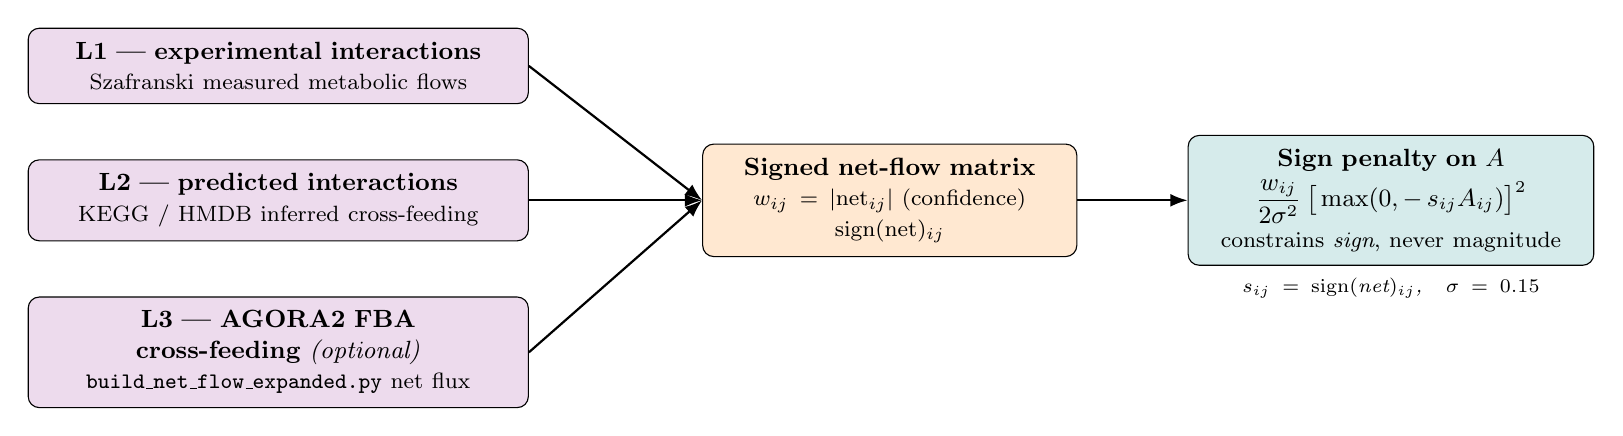
\begin{tikzpicture}[node distance=7mm]
  \node[prior,text width=6.0cm] (l1)
    {\textbf{L1 --- experimental interactions}\\
     {\footnotesize Szafranski measured metabolic flows}};
  \node[prior,below=of l1,text width=6.0cm] (l2)
    {\textbf{L2 --- predicted interactions}\\
     {\footnotesize KEGG / HMDB inferred cross-feeding}};
  \node[prior,below=of l2,text width=6.0cm] (l3)
    {\textbf{L3 --- AGORA2 FBA cross-feeding} \emph{(optional)}\\
     {\footnotesize \texttt{build\_net\_flow\_expanded.py} net flux}};

  \node[proc,right=22mm of l2,text width=4.4cm] (net)
    {\textbf{Signed net-flow matrix}\\
     {\footnotesize $w_{ij}=|\text{net}_{ij}|$ (confidence)}\\
     {\footnotesize $\operatorname{sign}(\text{net})_{ij}$}};

  \node[model,right=14mm of net,text width=4.8cm] (pen)
    {\textbf{Sign penalty on $A$}\\[2pt]
     $\dfrac{w_{ij}}{2\sigma^{2}}\,\big[\max(0,-\,s_{ij}A_{ij})\big]^{2}$\\[2pt]
     {\footnotesize constrains \emph{sign}, never magnitude}};

  \draw[flow] (l1.east) -- (net.west);
  \draw[flow] (l2.east) -- (net.west);
  \draw[flow] (l3.east) -- (net.west);
  \draw[flow] (net) -- (pen);

  \node[lbl,below=1mm of pen,text width=4.8cm,align=center]
    {$s_{ij}=\operatorname{sign}(\text{net})_{ij}$,\quad $\sigma=0.15$};
\end{tikzpicture}

% =============================================================== FIGURE 4 ====
% The four ODE attractors as a 2x2 quadrant.
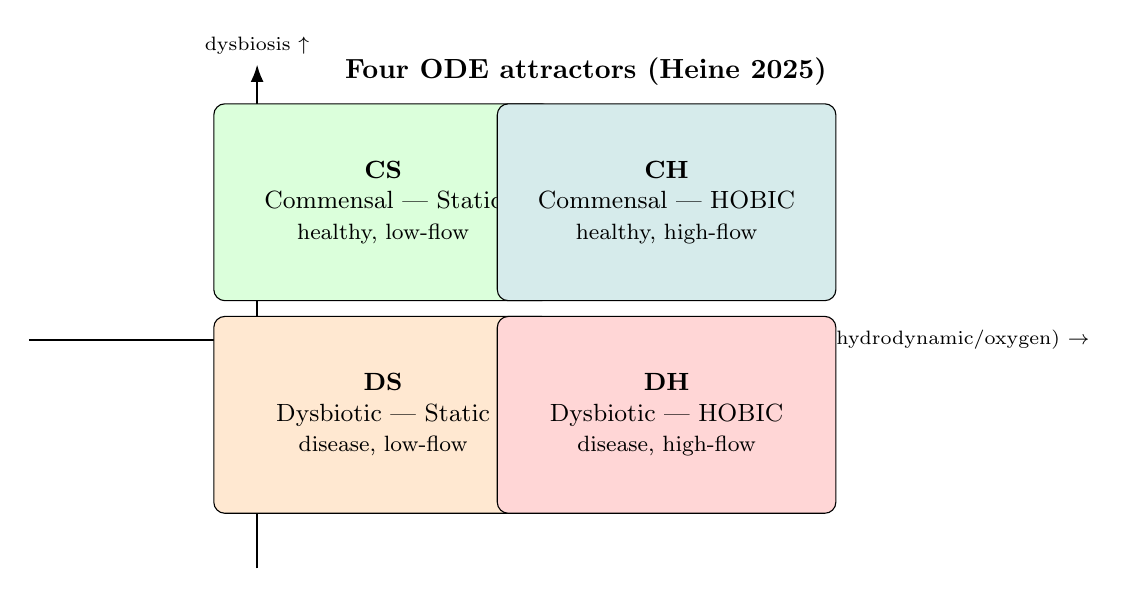
\begin{tikzpicture}[
    quad/.style={draw,rounded corners,minimum width=4.3cm,minimum height=2.5cm,
                 align=center,font=\small,inner sep=6pt},
  ]
  % axis lines
  \draw[flow] (-0.2,-3.1) -- (-0.2,3.3) node[above,font=\scriptsize]{dysbiosis $\uparrow$};
  \draw[flow] (-3.1,-0.2) -- (5.9,-0.2) node[right,font=\scriptsize]{HOBIC (hydrodynamic/oxygen) $\rightarrow$};

  \node[quad,fill=green!14]  (cs) at (1.4, 1.55)
    {\textbf{CS}\\ Commensal --- Static\\{\footnotesize healthy, low-flow}};
  \node[quad,fill=teal!16]   (ch) at (5.0, 1.55)
    {\textbf{CH}\\ Commensal --- HOBIC\\{\footnotesize healthy, high-flow}};
  \node[quad,fill=orange!18] (ds) at (1.4,-1.15)
    {\textbf{DS}\\ Dysbiotic --- Static\\{\footnotesize disease, low-flow}};
  \node[quad,fill=red!16]    (dh) at (5.0,-1.15)
    {\textbf{DH}\\ Dysbiotic --- HOBIC\\{\footnotesize disease, high-flow}};

  \node[font=\bfseries,above=1mm of ch.north east,anchor=south east]
    {Four ODE attractors (Heine 2025)};
\end{tikzpicture}

\end{document}
